% =====================================================================
\section{Background and Methods}
\label{sec:background}
% =====================================================================

We introduce Shapley explanation and the notation for the four choices underlying a given explanation (Figure~\ref{fig:overview}): the \emph{players} (\S\ref{sec:bg-players}), the \emph{imputation} (\S\ref{sec:bg-imputation}), the \emph{ground truth} (\S\ref{sec:bg-gt}), and the \emph{metric} (\S\ref{sec:bg-metrics}). MotionBench-XAI varies each choice independently. A glossary in Table~\ref{tab:notation} lists the full notation.

\subsection{Shapley values on spatiotemporal data}
\label{sec:bg-shapley}

A spatiotemporal instance is a tensor $\x \in \mathbb{R}^{J \times F \times T}$:
$J$ spatial units (skeleton joints, ECG leads, frequency bands), $F$ coordinates per unit (e.g.\ $F{=}3$ for $x,y,z$ positions), and $T$ time frames.  A trained classifier $\clf : \mathbb{R}^{J \times F \times T} \to \mathbb{R}$ maps $\x$ to a prediction, and the goal of an attribution is
to divide attribution for that prediction among parts of $\x$.

Shapley attribution \citep{lundberg2017unified} formalizes this as a cooperative game. A \emph{player set} $\Pset = \{1, \dots, \np\}$ partitions the entries of $\x$ into $\np$ disjoint groups (players).  For a coalition of players $\coal \subseteq \Pset$, the \emph{value function}, $\val$, evaluates the model on the instance with the players outside $\coal$ hidden:
\begin{equation}
  \val(\coal) \;=\; \clf\!\left(\fillx{\coal}\right),
  \label{eq:value}
\end{equation}
where $\fillx{\coal}$ denotes $\x$ with the entries of players in $\coal$ kept and all other entries replaced by an \emph{imputation} (defined in \S\ref{sec:bg-imputation}). We write $\bar{\coal} = \Pset \setminus \coal$ for the hidden players, $\x_{\coal}$ for the visible entries, and $\x_{\bar{\coal}}$ for the hidden block, so that $\fillx{\coal}$ is assembled from $\x_{\coal}$ and an imputation $\tilde{\x}_{\bar{\coal}}$ of the rest.
When the imputer is random, MotionBench-XAI draws $R$ imputations and averages them into one completion, $\tilde{\x}_{\bar{\coal}} = \frac{1}{R} \sum_{r=1}^{R} \tilde{\x}^{[r]}_{\bar{\coal}}$. Hence, we evaluate the classifier only once on the averaged fill $\tilde{\x}_{\bar{\coal}}$. Every stochastic imputer uses the same draw count, $R{=}5$ on the synthetic suite and $R{=}1$ on the real datasets (Appendix~\ref{app:coalition_protocol}). Every game value is therefore reproducible. The ground truths of
\S\ref{sec:bg-gt} replace the averaged draws with the exact conditional or
marginal mean, the $R \to \infty$ limit of this average.
% When the imputer is random, MotionBench-XAI draws $R$ imputations, fix them in advance, and average them into one completion, $\tilde{\x}_{\bar{\coal}} = \frac{1}{R} \sum_{r=1}^{R} \tilde{\x}^{[r]}_{\bar{\coal}}$.
% Hence, we evaluate the classifier only once on the averaged fill $\tilde{\x}_{\bar{\coal}}$. Every stochastic imputer uses the same draw count $R{=}5$. 

% Every Shapley value is therefore deterministic, meaning the ground truths of \S\ref{sec:bg-gt} are exactly computable.  

The Shapley value \citep{shapley1953value} of player $i$ is its average marginal contribution over all possible coalitions of players in $\Pset$,
\begin{equation}
  \shap_i \;=\; \sum_{\coal \subseteq \Pset \setminus \{i\}}
  \frac{|\coal|!\,(\np - |\coal| - 1)!}{\np!}
  \left[\val(\coal \cup \{i\}) - \val(\coal)\right].
  \label{eq:shapley}
\end{equation}

We write $\shap = (\shap_1, \dots, \shap_{\np})^{\!\top} \in \mathbb{R}^{\np}$ for the vector of Shapley values across all $\np$ players. Exact enumeration is exponential in $\np$. All methods in this paper estimate Eq.~\ref{eq:shapley} with KernelSHAP \citep{lundberg2017unified}, a weighted least-squares regression over sampled coalitions. We write $\shaphat \in \mathbb{R}^{\np}$ for the KernelSHAP estimate. We hold this estimator fixed across all KernelSHAP methods, evaluating the same number of coalitions throughout (Appendix~\ref{app:coalition_protocol}).
The temporal SHAP baselines run their reference implementations
(\S\ref{sec:bg-imputation}), so their rows also reflect their own estimators.

\subsection{What can a player be?}
\label{sec:bg-players}

The player set $\Pset$ decides how the input features will be preemptively divided before attributions are assigned (Figure~\ref{fig:overview}, second column). Figure~\ref{fig:players} shows the three families of players MotionBench-XAI evaluates on an example skeleton sequence. In every family, a player always includes all $F$ coordinates of the entries it covers. \textbf{Temporal
players} $\Pset_{\mathrm{temp}}$ cut the $T$ frames into $K$ uniform windows, and each window is one player ($\np = K$): this is the player set of temporal SHAP methods. \textbf{Spatial players} $\Pset_{\mathrm{joint}}$ make each spatial unit one player ($\np = J$). \textbf{Spatiotemporal players}
$\Pset_{\mathrm{cell}}$ combines the two, one player per joint $\times$ window cell ($\np = J \times K$). For example, on the CARE-PD gait data, the same
instance has $K=4$ windows, $J=17$ joints, which gives $M=68$ spatiotemporal players, also called cells.

\begin{figure}[t]
  \centering
  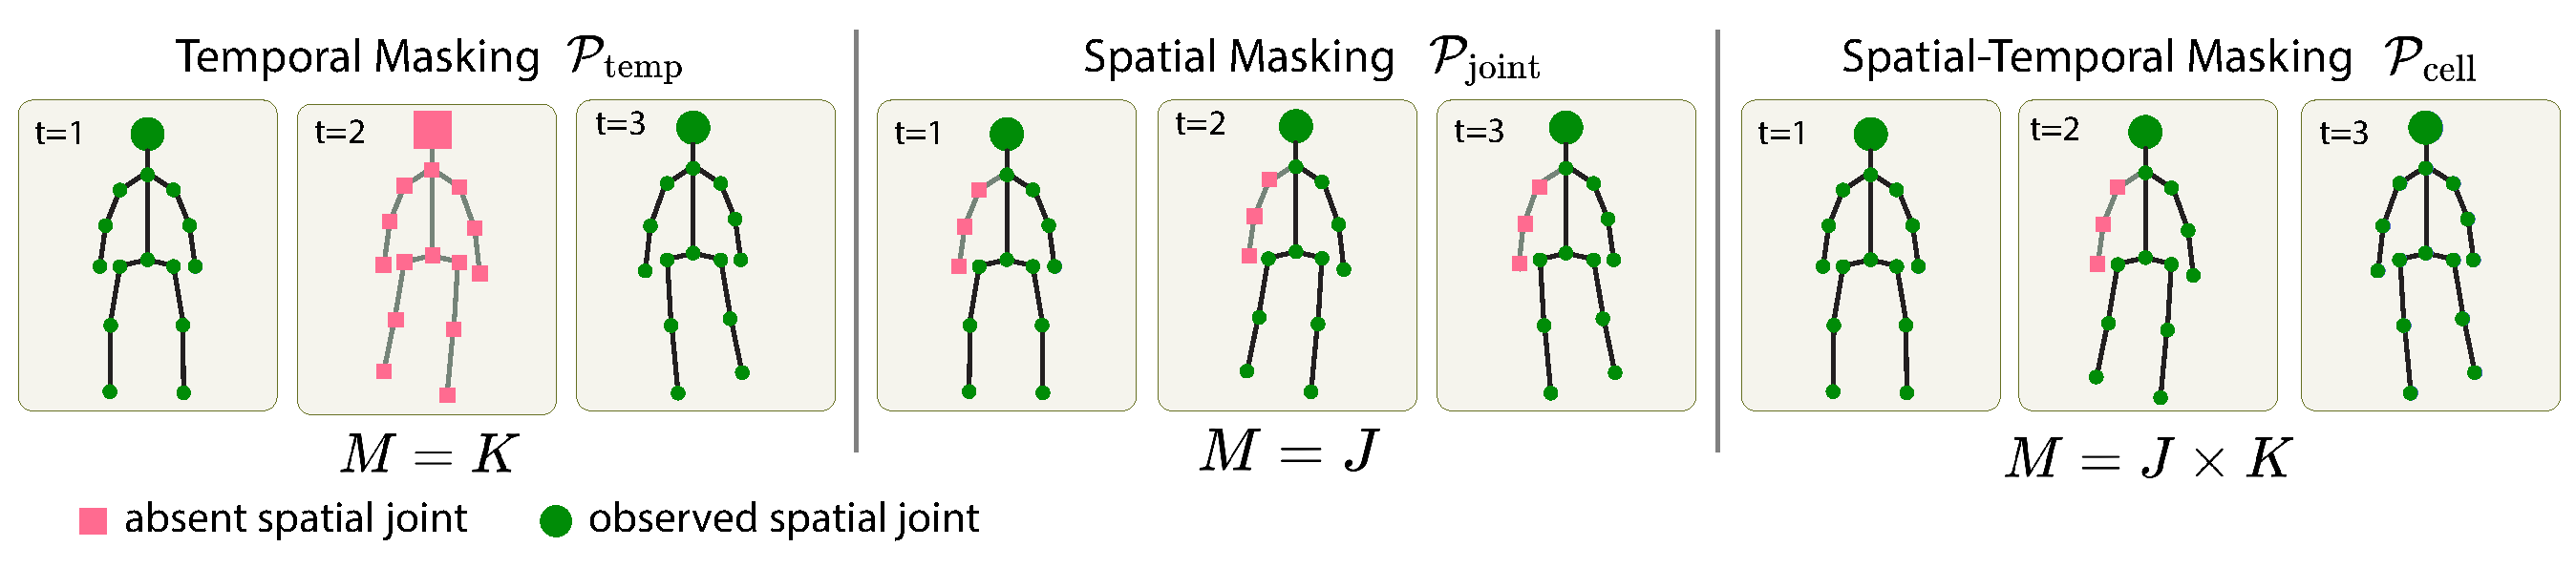
\includegraphics[width=\linewidth]{figures/spatio_temporal_shap_figure.pdf}
  \caption{\textbf{What can a player be?}  The three player sets, shown as
  masking on a skeleton sequence: a time window ($\Pset_{\mathrm{temp}}$), a spatial joint ($\Pset_{\mathrm{joint}}$), or a joint$\times$window cell
  ($\Pset_{\mathrm{cell}}$).}
  \label{fig:players}
\end{figure}

\subsection{What can an imputation be?}
\label{sec:bg-imputation}

Once we have our players, Eq.~\ref{eq:value} requires masking some of these players turn by turn. To avoid having to modify the model being explained, the masked players need to be imputed by some other value. Writing $x_i$ for the entries of a single hidden player $i \in \bar{\coal}$, MotionBench-XAI considers three families of methods (Figure~\ref{fig:overview}, third column). 

\textbf{Standard (off manifold).}  The hidden player is replaced by a value that ignores the rest of the sequence: zeros ($x_i = 0$), the training mean
($x_i = \mathbb{E}[x_i]$), or a draw from the marginal ($x_i \sim P(x_i)$,
copied from another sequence in the evaluation pool). These define the
methods KS-Zero and KS-Mean \citep{lundberg2017unified}, KS-Marginal \citep{aas2021explaining}, and KS-Empirical \citep{aas2021explaining,redelmeier2020explaining}. KS-Empirical refines KS-Marginal by copying values from the sequences most similar to the explained one, weighted by a kernel. These imputations are cheap and model-agnostic but off manifold \citep{frye2021shapley}. On human skeleton data, for example, they can produce anatomically impossible motion.

\textbf{Temporal (on the temporal manifold).} WindowSHAP
\citep{NAYEBI2023104438} and TimeSHAP \citep{bento2021timeshap} keep the
standard zero fill. They distinguish themselves by cleverly picking temporal players to begin with: fixed windows (WindowSHAP-S), adaptively split windows (WindowSHAP-D), or per-event scoring with pruning (TimeSHAP). We evaluate them at temporal players only, aggregating per-timestep attributions into the $K$ uniform windows.

\textbf{Generative (on manifold).}  This family uses a conditional model to impute the hidden player from the visible ones, $x_i \sim P(x_i \mid \x_{\coal})$. KS-VAEAC (\citealp{olsen2022using,ivanov2018variational}) and KS-Flow use learned conditional models; their formulations are given in
Appendix~\ref{app:imputer_detail}.
We build KS-Flow for this benchmark so that the generative family contains two learned imputers of different strength. It mirrors KS-VAEAC except that it replaces the VAEAC generative model with a flow matching model \citep{lipman2023flow}. KS-Gauss (\citealp{aas2021explaining}) is the closed-form Gaussian conditional, with no learned components. These imputers stay near the data manifold but are learned or assumption-bound, hence imperfect. % KS-Oracle draws from the \emph{exact} conditional law, available only on our synthetic datasets (\S\ref{sec:bg-gt}).

\subsection{What can a ground truth be?}
\label{sec:bg-gt}
In cooperative game theory, a game is defined as a rule that assigns a score to every coalition of players. In our setting, that rule is Eq.~\ref{eq:value}. The score of a coalition is the model's prediction on the input with the remaining players imputed, so the imputation is part of the rule. When we change how the hidden players are filled, the same
coalition receives a different score. We are then playing a different game, and Eq.~\ref{eq:shapley} assigns different attributions to the same input. In this work, two games stand out. If we fill the hidden players with their marginal expectation $\mathbb{E}[\x_{\bar{\coal}}]$, we play the \emph{marginal game}. If we instead fill them with their conditional expectation $\mathbb{E}[\x_{\bar{\coal}} \mid \x_{\coal}]$, we play the \emph{conditional game}~\citep{janzing2020feature,chen2020true}. The standard and temporal imputers of \S\ref{sec:bg-imputation} approximate the marginal game. The generative imputers approximate the conditional game. A \textit{ground truth Shapley value} solves a game exactly, using the expectation itself instead of an estimate of it. 

% Both are mean-imputation games. Conventional conditional SHAP instead
% averages the model output over imputations \citep{aas2021explaining},
% which differs for nonlinear models. Every method here runs under the
% shared mean-imputation protocol of \S\ref{sec:bg-shapley}.

On synthetic data drawn from a well-chosen distribution, both expectations are available in closed form for every coalition. We can therefore compute both ground truths exactly (see App.~\ref{app:oracle_proofs}). For player sets with at most 12 players we enumerate every coalition, so the ground-truth Shapley values carry no error at all. For larger player sets we solve the same exact games on large sampled coalition designs and measure the remaining target error directly Importantly, since the two exact imputations differ, the two ground truths assign different attributions. MotionBench-XAI grades each imputer method against the ground truth of its own game, which we call \emph{game-matched} grading. Where possible, we also report the standard convention of grading everything against $\gtman$. On real data, neither expectation is knowable. 

% Each imputer family is an estimator of the \emph{estimand} used in Eq.~\ref{eq:value}. Standard imputers approximate this estimand with the marginal expectation $\mathbb{E}[x_i]$ and are as such typically considered off-manifold. Generative imputers approximate this estimand using a conditional expectation $\mathbb{E}[x_i \mid \x_{\coal}]$ and are considered on-manifold. A \textit{ground truth Shapley value} is obtained by using the known estimand itself rather than an estimate of it. In summary:
% \begin{align}
%   \gtstd &: \text{Shapley values of the game with the exact marginal imputation } \mathbb{E}[x_i],\\
%   \gtman &: \text{Shapley values of the game with the exact conditional imputation } \mathbb{E}[x_i \mid \x_{\coal}].
% \end{align}
% On real data neither estimand is knowable. On synthetic data drawn from a well-chosen distribution, both are available in closed form for every coalition. Hence, both the marginal and the conditional games are deterministic and both ground truths are exactly computable (see Proposition~\ref{prop:oracle} and
% Appendix~\ref{app:oracle_proofs}). Importantly, since the two exact imputations differ, the two ground truths assign different attributions. This shifting ground truth is a fundamental property of Shapley attributions and is critical to consider in practice. MotionBench-XAI grades each imputer method against the ground truth of its own family, which we call \emph{game-matched} grading. Where possible, we also report the standard convention of grading everything against $\gtman$.

\subsection{What metric do we use to score the quality of an explanation?}
\label{sec:bg-metrics}

\paragraph{With ground truth (synthetic data).} Following
\citet{aas2021explaining,olsen2022using}, MotionBench-XAI reports two error criteria (EC, following \citet{olsen2022using}):
\begin{equation}
  \ECone = \tfrac{1}{\np}\,\big\lVert \shaphat - \shap^{\star} \big\rVert_1
  \qquad\text{and}\qquad
  \ECthree = 1 - r\!\left(\shaphat,\, \shap^{\star}\right),
\end{equation}
where $\shap^{\star}$ is the game-matched ground truth and $r$ is the Pearson
correlation per sequence. $\ECone$ is the mean absolute attribution error.
$\ECthree$ is its scale-invariant counterpart that measures how well the player attributions' order and weight match the ground truth. Lower is better for both.

\paragraph{Without ground truth (real data).} MotionBench-XAI uses the two standard deletion-based tests. \emph{Faithfulness correlation} \citep{bhatt2020evaluating} correlates the summed attributions of hidden players with the model's performance drop across coalitions. \emph{PlayerAOPC} \citep{samek2017evaluating} removes players in decreasing-attribution order and records the model's response. Higher is better for both. For both metrics, $\val(\coal)$ is computed with each method's own imputer, on the same coalitions. $\ECthree$ and faithfulness can be compared across player sets. However, $\ECone$ and PlayerAOPC scale with the number of players, so their values compare only within one player set.
